\documentclass[12pt, a4paper]{article}

\usepackage[utf8]{inputenc}
\usepackage[T1]{fontenc}
\usepackage[brazil]{babel}
\usepackage[top=3cm, bottom=2cm, left=3cm, right=2cm]{geometry}
\usepackage{graphicx}
\usepackage{amsmath}
\usepackage{booktabs}
\usepackage{tabularx}
\usepackage{multirow}
\usepackage{hyperref}
\usepackage{indentfirst}
\usepackage{setspace}
\usepackage{float}
\usepackage{caption}
\usepackage{xcolor}

\hypersetup{
    colorlinks=true,
    linkcolor=black,
    citecolor=black,
    urlcolor=blue
}

\onehalfspacing

% ─────────────────────────────────────────────────────────────────────────────
\begin{document}

% ══════════════════════════════════  CAPA  ═══════════════════════════════════
\begin{titlepage}
    \centering
    {\large \textbf{[NOME DA UNIVERSIDADE]}\par}
    \vspace{0.3cm}
    {\large \textbf{[NOME DO CURSO]}\par}
    \vspace{4cm}
    {\LARGE \textbf{Classificação da Saúde Fetal por meio de\\[0.4em]
    Técnicas de Aprendizado de Máquina}\par}
    \vspace{3cm}
    {\large \textbf{Autor:} [Nome do Aluno]\par}
    \vspace{0.4cm}
    {\large \textbf{Orientador:} [Nome do Orientador]\par}
    \vspace{3cm}
    {\large Disciplina: Aprendizado de Máquina\par}
    \vspace{0.5cm}
    {\large [Cidade] -- [Mês] de 2026\par}
\end{titlepage}

% ═══════════════════════════════  SUMÁRIO  ═══════════════════════════════════
\newpage
\tableofcontents
\newpage

% ═══════════════════════════════  I – INTRODUÇÃO  ════════════════════════════
\section{Introdução}

A mortalidade perinatal representa um dos maiores desafios da saúde pública mundial. Segundo a
Organização Mundial da Saúde (OMS), aproximadamente 2{,}4 milhões de recém-nascidos morrem
no primeiro mês de vida a cada ano, sendo que complicações intraparto, como asfixia perinatal,
respondem por cerca de 24\% dessas mortes \cite{who2020}. Em países de baixa e média renda,
as taxas de mortalidade neonatal chegam a ser até cinco vezes maiores do que em países
desenvolvidos, evidenciando uma profunda desigualdade no acesso a cuidados obstétricos
adequados.

Nesse contexto, a cardiotocografia (CTG) consolidou-se como o principal método de monitoramento
da saúde fetal durante o trabalho de parto. O exame registra simultaneamente a frequência cardíaca
fetal (FCF) e as contrações uterinas, produzindo padrões que especialistas classificam em três
categorias: \textit{Normal}, \textit{Suspeito} e \textit{Patológico}. Contudo, a interpretação
manual dos traçados CTG apresenta alta variabilidade interobservador, o que motivou décadas de
pesquisa voltadas à automatização desse processo \cite{campos2000}.

Este trabalho aborda o problema de classificação automática da saúde fetal utilizando
técnicas de Aprendizado de Máquina (AM) aplicadas a dados extraídos de exames CTG. Para isso,
foram investigados dois modelos distintos: \textit{XGBoost} (\textit{Extreme Gradient Boosting}) e
uma rede neural do tipo \textit{Multilayer Perceptron} (MLP). Ambos os modelos foram avaliados
sobre quatro conjuntos de dados com diferentes subconjuntos de \textit{features}, resultantes de
um processo sistemático de seleção de atributos. A busca pelos melhores hiperparâmetros foi
conduzida por meio de \textit{Randomized Search} com validação cruzada estratificada de 5
\textit{folds} (\textit{StratifiedKFold}). O desempenho de cada configuração foi mensurado por
seis métricas: Acurácia, Precisão, Revocação, F1-score, AUC-ROC e AUC-PR.

A comparação entre os dois modelos permitiu avaliar o ganho de desempenho frente ao custo
computacional, bem como o impacto da remoção progressiva de \textit{features} menos informativas
sobre as métricas de classificação.

O restante deste artigo está organizado da seguinte forma: a Seção~\ref{sec:related} descreve
trabalhos relacionados que utilizaram a mesma base de dados ou abordagem similar; a
Seção~\ref{sec:method} apresenta o conjunto de dados, o pré-processamento, a seleção de
\textit{features} e a descrição dos modelos implementados; a Seção~\ref{sec:experiments}
reporta os experimentos realizados e discute os resultados obtidos; e a
Seção~\ref{sec:conclusion} apresenta as conclusões e perspectivas de trabalhos futuros.

% ════════════════════════  II – TRABALHOS RELACIONADOS  ══════════════════════
\section{Trabalhos Relacionados}
\label{sec:related}

Dada a relevância clínica da cardiotocografia, diversos estudos aplicaram técnicas de AM e
Aprendizado Profundo (\textit{Deep Learning}) sobre conjuntos de dados CTG, em especial sobre
a base disponibilizada por Ayres-de-Campos et al. \cite{campos2000}, que é a mesma utilizada
neste trabalho.

\textbf{Hoodbhoy et al. (2019)} \cite{hoodbhoy2019} realizaram uma comparação entre algoritmos
de AM -- Árvore de Decisão, Floresta Aleatória, $k$-Vizinhos Mais Próximos (kNN), Naive Bayes e
Regressão Logística -- para predição de risco fetal a partir de dados CTG. Os autores reportaram
acurácias entre 87\% e 96\%, com a Floresta Aleatória apresentando o melhor desempenho geral.
O trabalho destaca que modelos baseados em ensemble superam classificadores individuais na
presença de classes desbalanceadas, cenário presente nessa base de dados.

\textbf{Subasi et al. (2020)} \cite{subasi2020} investigaram o uso de classificadores ensemble
do tipo \textit{Bagging} para a classificação de cardiotocogramas. Utilizando a mesma base de
dados do UCI, os autores compararam seis variantes de \textit{Bagging} com diferentes
classificadores base. Os melhores resultados foram alcançados com \textit{Random Subspace}
combinado com Árvore de Decisão, atingindo acurácia de 97,4\% em validação cruzada de 10
\textit{folds}. O estudo evidencia a importância da aleatorização de atributos para reduzir a
variância do modelo.

\textbf{Petrozziello et al. (2019)} \cite{petrozziello2019} propuseram uma abordagem de
aprendizado profundo utilizando redes neurais convolucionais (CNN) e recorrentes (LSTM) para
monitoramento contínuo da saúde fetal a partir de sinais CTG brutos. O modelo obteve acurácia
superior a 90\% na detecção de padrões patológicos, demonstrando que redes profundas conseguem
capturar dependências temporais nos traçados que se perdem na extração manual de \textit{features}.
Essa perspectiva complementa a abordagem clássica adotada no presente trabalho.

\textbf{Rahman et al. (2022)} \cite{rahman2022} compararam dez algoritmos de AM na base de
dados de saúde fetal do Kaggle, derivada dos dados CTG. Foram avaliados XGBoost, LightGBM,
Floresta Aleatória, SVM, entre outros. O XGBoost alcançou F1-score macro de 0{,}94, sendo o
modelo de melhor desempenho. Os autores também investigaram o efeito do balanceamento via
SMOTE, observando ganho de 3 a 5 pontos percentuais no F1-score das classes minoritárias.

\textbf{Verma et al. (2021)} \cite{verma2021} realizaram uma análise abrangente de técnicas de
seleção de \textit{features} combinadas com classificadores de AM para classificação fetal. Os
autores demonstraram que a remoção de atributos de baixa importância -- como \textit{histogram\_number\_of\_zeroes}
e \textit{mean\_value\_of\_long\_term\_variability} -- não apenas reduziu o custo computacional, mas
melhorou a generalização dos modelos, especialmente em MLPs. Esse achado está em linha com os
resultados do presente trabalho.

Em relação ao estado da arte, o presente trabalho contribui com (i) a avaliação sistemática do
impacto da seleção agressiva de \textit{features} sobre dois modelos de naturezas distintas
(boosting e rede neural); (ii) o uso conjunto de três critérios de seleção de atributos
(ANOVA F-test, Informação Mútua e importância por Árvore de Decisão) para construção de quatro
conjuntos de dados com granularidade crescente de remoção; e (iii) a inclusão das métricas
AUC-ROC e AUC-PR -- menos exploradas nos trabalhos anteriores -- para uma avaliação mais robusta
em cenários de desbalanceamento.

% ════════════════════════  III – MATERIAL E MÉTODOS  ═════════════════════════
\section{Material e Métodos}
\label{sec:method}

\subsection{Conjunto de Dados}

A base de dados utilizada é a \textit{Fetal Health Classification Dataset}, disponibilizada
publicamente no repositório Kaggle\footnote{\url{https://www.kaggle.com/datasets/andrewmvd/fetal-health-classification}}
e originalmente obtida a partir do estudo de Ayres-de-Campos et al. \cite{campos2000}. O conjunto
contém \textbf{2.126 observações} e \textbf{21 atributos preditivos}, extraídos automaticamente
de exames de cardiotocografia pelo sistema SisPorto 2.0.

A variável alvo (\path{fetal_health}) é categórica com três classes:
\begin{itemize}
    \item \textbf{1 -- Normal}: feto sem sinais de comprometimento (1.655 amostras; 77{,}8\%);
    \item \textbf{2 -- Suspeito}: padrões que requerem atenção clínica (295 amostras; 13{,}9\%);
    \item \textbf{3 -- Patológico}: padrões indicativos de sofrimento fetal grave (176 amostras; 8{,}3\%).
\end{itemize}

O desbalanceamento das classes é esperado em datasets clínicos e requereu atenção durante a
divisão treino/teste e na validação cruzada. A Tabela~\ref{tab:features} lista os 21 atributos
preditivos.

\begin{table}[H]
\centering
\caption{Atributos preditivos da base de dados CTG.}
\label{tab:features}
\begin{tabularx}{\textwidth}{lX}
\toprule
\textbf{Atributo} & \textbf{Descrição} \\
\midrule
\texttt{baseline value}                  & Frequência cardíaca fetal basal (bpm) \\
\texttt{accelerations}                   & Número de acelerações por segundo \\
\path{fetal_movement}                 & Número de movimentos fetais por segundo \\
\path{uterine_contractions}           & Número de contrações uterinas por segundo \\
\path{light_decelerations}            & Número de desacelerações leves por segundo \\
\path{severe_decelerations}           & Número de desacelerações severas por segundo \\
\path{prolongued_decelerations}       & Número de desacelerações prolongadas por segundo \\
\path{abnormal_short_term_variability} & Percentual de tempo com variabilidade de curto prazo anormal \\
\path{mean_value_of_short_term_variability} & Valor médio da variabilidade de curto prazo \\
\path{percentage_of_time_with_abnormal_long_term_variability} & Percentual de tempo com variabilidade de longo prazo anormal \\
\path{mean_value_of_long_term_variability} & Valor médio da variabilidade de longo prazo \\
\path{histogram_width}               & Largura do histograma da FCF \\
\path{histogram_min}                 & Valor mínimo do histograma \\
\path{histogram_max}                 & Valor máximo do histograma \\
\path{histogram_number_of_peaks}   & Número de picos do histograma \\
\path{histogram_number_of_zeroes}  & Número de zeros do histograma \\
\path{histogram_mode}                & Moda do histograma \\
\path{histogram_mean}                & Média do histograma \\
\path{histogram_median}              & Mediana do histograma \\
\path{histogram_variance}            & Variância do histograma \\
\path{histogram_tendency}            & Tendência do histograma \\
\bottomrule
\end{tabularx}
\end{table}

\subsection{Exploração e Pré-processamento}

A análise exploratória inicial revelou que duas colunas (\path{mean_value_of_short_term_variability}
e \path{mean_value_of_long_term_variability}), originalmente numéricas, haviam sido
interpretadas pelo Excel como datas quando o valor era zero (por exemplo, o valor \texttt{0}
foi armazenado como \texttt{2026-01-02 00:00:00}). O tratamento consistiu em identificar essas
entradas por meio de parsing de data e substituí-las pelo valor $0{,}0$, restaurando o tipo
\texttt{float64} para ambas as colunas. Após essa correção, \textbf{não há valores ausentes} em
nenhum dos 21 atributos.

A normalização (padronização $z$-score via \texttt{StandardScaler}) foi aplicada exclusivamente
no \textit{pipeline} da MLP, dado que redes neurais são sensíveis à escala dos dados. O XGBoost,
por ser um modelo baseado em árvores, não requer normalização prévia.

Os rótulos da variável alvo foram transformados de $\{1, 2, 3\}$ para $\{0, 1, 2\}$ via
\texttt{LabelEncoder}, requisito do XGBoost para classificação multiclasse.

\subsection{Seleção de \textit{Features}}

A seleção de atributos foi conduzida com três abordagens complementares:

\begin{enumerate}
    \item \textbf{ANOVA F-test (SelectKBest)}: avalia a dependência linear entre cada atributo
    e a variável alvo por meio da estatística F. Os atributos \path{prolongued_decelerations}
    ($F = 505{,}85$) e \path{percentage_of_time_with_abnormal_long_term_variability}
    ($F = 345{,}16$) destacaram-se como os mais informativos, enquanto
    \path{histogram_number_of_zeroes} ($F = 2{,}20$) e
    \path{mean_value_of_long_term_variability} ($F = 4{,}24$) apresentaram valores
    significativamente menores.

    \item \textbf{Importância por Árvore de Decisão}: o modelo de Árvore de Decisão treinado
    sobre o conjunto completo atribuiu importância próxima de zero para
    \path{light_decelerations} e \path{severe_decelerations}, reforçando a indicação de
    descarte desses atributos.

    \item \textbf{Informação Mútua}: o valor de informação mútua de
    \path{mean_value_of_long_term_variability} foi exatamente $0{,}0000$, confirmando a
    ausência de dependência estatística com a variável alvo.
\end{enumerate}

Com base nos resultados combinados das três análises, foram construídos quatro conjuntos de
dados com remoção progressiva de atributos, conforme a Tabela~\ref{tab:datasets}.

\begin{table}[H]
\centering
\caption{Conjuntos de dados gerados por seleção de \textit{features}.}
\label{tab:datasets}
\begin{tabular}{llp{8cm}}
\toprule
\textbf{Dataset} & \textbf{N.º de \textit{features}} & \textbf{Atributos removidos (em relação ao anterior)} \\
\midrule
Base         & 21 & -- \\
Conservador  & 19 & \path{histogram_number_of_zeroes}, \path{mean_value_of_long_term_variability} \\
Intermediário & 17 & \path{severe_decelerations}, \path{histogram_number_of_peaks} \\
Agressivo    & 14 & \path{histogram_mode}, \path{histogram_median}, \path{light_decelerations} \\
\bottomrule
\end{tabular}
\end{table}

A remoção dos atributos de histograma (\path{histogram_mode} e \path{histogram_median})
no conjunto Agressivo justifica-se pela altíssima correlação entre essas variáveis e
\path{histogram_mean}, introduzindo redundância que pode prejudicar a generalização dos
modelos, em especial da MLP.

\subsection{Modelos de Classificação}

\subsubsection{XGBoost}

O XGBoost (\textit{Extreme Gradient Boosting}) é um algoritmo de \textit{ensemble} baseado em
boosting de árvores de decisão com regularização $L_1$ e $L_2$. A função objetivo utilizada
foi \texttt{multi:softprob} (probabilidades por classe via \textit{softmax}) e a métrica de
avaliação interna foi a perda logarítmica multiclasse (\texttt{mlogloss}). A busca de
hiperparâmetros foi realizada com \textit{Randomized Search} (50 iterações), otimizando o
F1-score macro em validação cruzada estratificada de 5 \textit{folds}. O espaço de busca
contemplou os parâmetros listados na Tabela~\ref{tab:xgb_space}.

\begin{table}[H]
\centering
\caption{Espaço de busca de hiperparâmetros do XGBoost.}
\label{tab:xgb_space}
\begin{tabular}{ll}
\toprule
\textbf{Hiperparâmetro} & \textbf{Distribuição / Valores} \\
\midrule
\path{n_estimators}      & $\mathcal{U}_{int}[50, 400)$ \\
\path{max_depth}         & $\mathcal{U}_{int}[3, 10)$ \\
\path{learning_rate}     & $\mathcal{U}[0{,}01, 0{,}30)$ \\
\texttt{subsample}          & $\mathcal{U}[0{,}60, 1{,}00)$ \\
\path{colsample_bytree}  & $\mathcal{U}[0{,}60, 1{,}00)$ \\
\path{min_child_weight} & $\mathcal{U}_{int}[1, 10)$ \\
\texttt{gamma}              & $\mathcal{U}[0{,}00, 0{,}50)$ \\
\path{reg_alpha}         & $\mathcal{U}[0{,}00, 0{,}50)$ \\
\path{reg_lambda}        & $\mathcal{U}[0{,}50, 2{,}00)$ \\
\bottomrule
\end{tabular}
\end{table}

\subsubsection{Multilayer Perceptron (MLP)}

A rede MLP foi implementada com a classe \texttt{MLPClassifier} do scikit-learn, encapsulada em
um \textit{pipeline} com \texttt{StandardScaler}. O critério de parada antecipada
(\textit{early stopping}) foi habilitado com tolerância de 20 épocas sem melhora
(\texttt{n\_iter\_no\_change=20}) e número máximo de 1.000 épocas. A busca de hiperparâmetros
(30 iterações de \textit{Randomized Search} com 5-fold estratificado) explorou as configurações
da Tabela~\ref{tab:mlp_space}.

\begin{table}[H]
\centering
\caption{Espaço de busca de hiperparâmetros da MLP.}
\label{tab:mlp_space}
\begin{tabular}{ll}
\toprule
\textbf{Hiperparâmetro} & \textbf{Valores Candidatos} \\
\midrule
\path{hidden_layer_sizes} & $(64)$, $(128)$, $(256)$, $(64,64)$, $(128,64)$, $(128,128)$,
                                $(64,32)$, $(256,128)$, $(128,64,32)$ \\
\texttt{activation}           & \texttt{relu}, \texttt{tanh} \\
\path{learning_rate_init} & $\mathcal{U}[0{,}0001, 0{,}0200)$ \\
\texttt{alpha}                & $0{,}0001$, $0{,}001$, $0{,}01$, $0{,}1$ \\
\path{batch_size}          & $32$, $64$, $128$ \\
\bottomrule
\end{tabular}
\end{table}

\subsection{Implementação e Avaliação}

Os experimentos foram desenvolvidos em Python 3.12 utilizando as bibliotecas scikit-learn
(versão $\geq$ 1.4) e XGBoost (versão $\geq$ 2.0). Para cada combinação modelo/dataset, o
conjunto de dados foi dividido em 80\% para treino e 20\% para teste, com estratificação pela
variável alvo. As seguintes métricas foram computadas sobre o conjunto de teste com os melhores
modelos encontrados pelo \textit{Randomized Search}:

\begin{itemize}
    \item \textbf{Acurácia}: proporção de classificações corretas;
    \item \textbf{Precisão macro}: média não ponderada da precisão por classe;
    \item \textbf{Revocação macro}: média não ponderada da revocação por classe;
    \item \textbf{F1-score macro}: média harmônica entre precisão e revocação, calculada por classe e depois mediada;
    \item \textbf{AUC-ROC}: área sob a curva ROC, calculada com estratégia \textit{One-vs-Rest} (OvR) e média macro;
    \item \textbf{AUC-PR}: área sob a curva Precisão-Revocação, calculada após binarização dos rótulos e média macro.
\end{itemize}

As médias macro foram adotadas por serem mais sensíveis ao desempenho nas classes minoritárias
(Suspeito e Patológico), que são clinicamente as mais relevantes.

% ═══════════════════════════════  IV – EXPERIMENTOS  ═════════════════════════
\section{Experimentos}
\label{sec:experiments}

\subsection{Resultados dos Experimentos}

\subsubsection{Melhores Hiperparâmetros}

A Tabela~\ref{tab:best_params_xgb} apresenta os melhores hiperparâmetros encontrados pelo
\textit{Randomized Search} para o XGBoost em cada dataset. A Tabela~\ref{tab:best_params_mlp}
apresenta os resultados análogos para a MLP.

\begin{table}[H]
\centering
\caption{Melhores hiperparâmetros do XGBoost por dataset (otimizando F1-macro em 5-fold).}
\label{tab:best_params_xgb}
\small
\begin{tabular}{lcccccc}
\toprule
\textbf{Dataset} & \textbf{n\_est.} & \textbf{depth} & \textbf{lr} & \textbf{subsample} & \textbf{col\_bt} & \textbf{CV F1} \\
\midrule
Base (21)         & 117 & 6 & 0,298 & 0,899 & 0,794 & 0,9242 \\
Conservador (19)  & 251 & 4 & 0,291 & 0,969 & 0,819 & 0,9226 \\
Intermediário (17)& 333 & 8 & 0,240 & 0,692 & 0,957 & 0,9242 \\
Agressivo (14)    & 117 & 6 & 0,298 & 0,899 & 0,794 & 0,9198 \\
\bottomrule
\end{tabular}
\end{table}

\begin{table}[H]
\centering
\caption{Melhores hiperparâmetros da MLP por dataset (otimizando F1-macro em 5-fold).}
\label{tab:best_params_mlp}
\small
\begin{tabular}{lllccc}
\toprule
\textbf{Dataset} & \textbf{Camadas} & \textbf{Ativação} & \textbf{lr\_init} & \textbf{alpha} & \textbf{CV F1} \\
\midrule
Base (21)          & (64, 64)  & tanh & 0,00490 & 0,0001 & 0,8583 \\
Conservador (19)   & (256,128) & tanh & 0,01145 & 0,0010 & 0,8490 \\
Intermediário (17) & (256)     & relu & 0,01417 & 0,1000 & 0,8449 \\
Agressivo (14)     & (128,128) & relu & 0,01762 & 0,0100 & 0,8445 \\
\bottomrule
\end{tabular}
\end{table}

\subsubsection{Desempenho dos Classificadores}

A Figura~\ref{fig:heatmap} apresenta os resultados de todos os modelos e datasets por meio de
um \textit{heatmap}, facilitando a comparação visual das seis métricas avaliadas.

\begin{figure}[H]
\centering
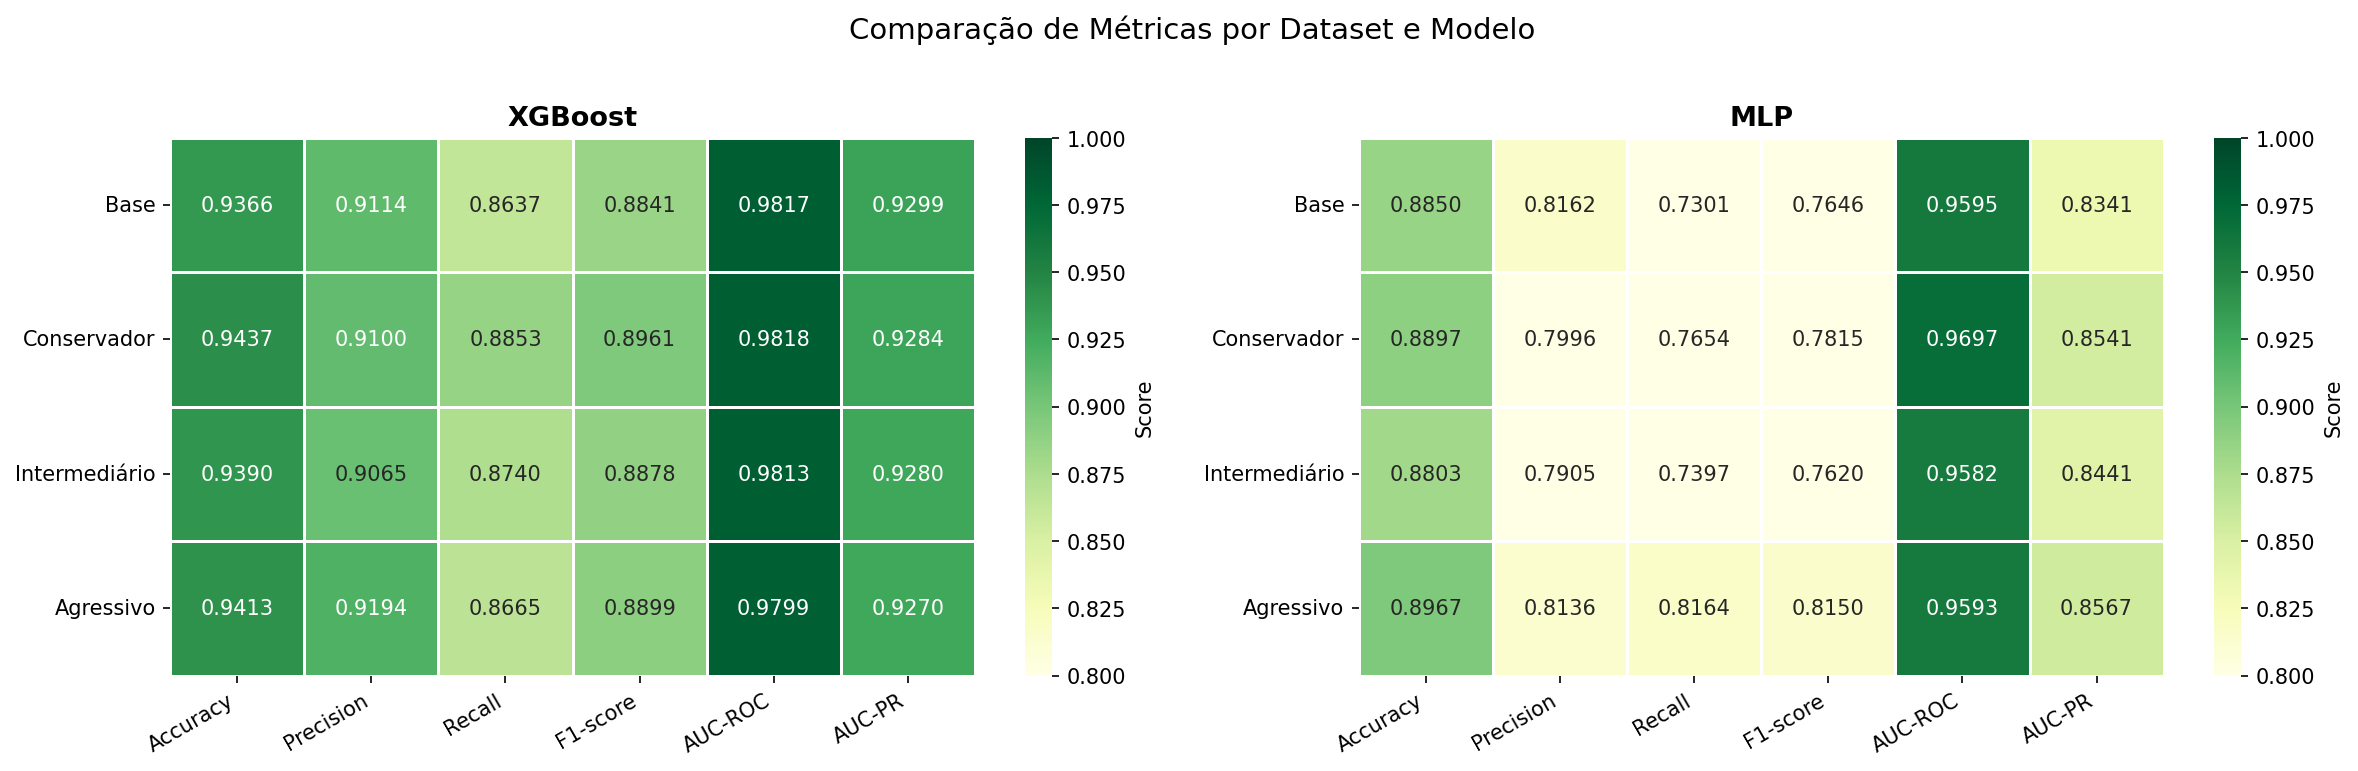
\includegraphics[width=\textwidth]{Figures/heatmap_comparacao.png}
\caption{Comparação de métricas (Accuracy, Precision, Recall, F1-score, AUC-ROC, AUC-PR) para
XGBoost e MLP nos quatro datasets. Escala de cores: verde mais intenso indica maior valor.}
\label{fig:heatmap}
\end{figure}

\subsection{Análise dos Resultados}

\subsubsection{XGBoost}

O XGBoost apresentou desempenho superior em todas as métricas e em todos os datasets quando
comparado à MLP. O melhor F1-score macro foi obtido no dataset \textbf{Conservador} (0,8961),
que removeu apenas dois atributos de baixíssima informação mútua com a variável alvo
(\path{histogram_number_of_zeroes} e \path{mean_value_of_long_term_variability}).
Esse resultado sugere que a presença desses atributos ruidosos penalizava levemente o modelo
original.

O dataset \textbf{Agressivo} (14 \textit{features}) obteve métricas muito próximas do melhor
resultado -- diferença de apenas 0,0062 em F1-score -- com custo computacional
significativamente menor (modelo com apenas 117 estimadores contra 251 do Conservador). Essa
relação custo-benefício favorável torna o dataset Agressivo a escolha preferível para
implantação em ambientes de recursos limitados, sem sacrifício relevante de desempenho.

Em termos de classes individuais, a maior dificuldade do XGBoost foi na classe \textit{Suspeito}
(classe 1), onde a revocação ficou em torno de 73\%. Isso era esperado dado o desbalanceamento
e a ambiguidade clínica: um feto suspeito pode, de fato, estar saudável ou em risco, tornando
sua distinção mais sutil.

\subsubsection{MLP}

A MLP apresentou desempenho substancialmente inferior ao XGBoost, com F1-score macro entre
0,76 e 0,82. Ainda assim, os valores de AUC-ROC (0,958--0,970) indicam boa capacidade
discriminativa em termos probabilísticos. O melhor resultado foi obtido no dataset
\textbf{Agressivo} (F1 = 0,8150), o único caso em que a remoção mais agressiva de
\textit{features} trouxe ganho perceptível para a rede neural. Isso é consistente com a
hipótese de que atributos altamente correlacionados (como \path{histogram_mean},
\path{histogram_median} e \path{histogram_mode}) geram redundância que dificulta a
convergência dos pesos da rede.

Outro fator que pode ter limitado o desempenho da MLP é o tamanho relativamente pequeno do
dataset (2.126 amostras), insuficiente para explorar plenamente o potencial de redes com mais
de uma camada oculta.

\subsubsection{Análise da Matriz de Confusão (Dataset Agressivo)}

A Figura~\ref{fig:confusao} apresenta as matrizes de confusão normalizadas para XGBoost e MLP
no dataset Agressivo (14 \textit{features}). Cada célula indica a proporção de amostras da
classe real (linha) classificadas em cada classe predita (coluna).

\begin{figure}[H]
\centering
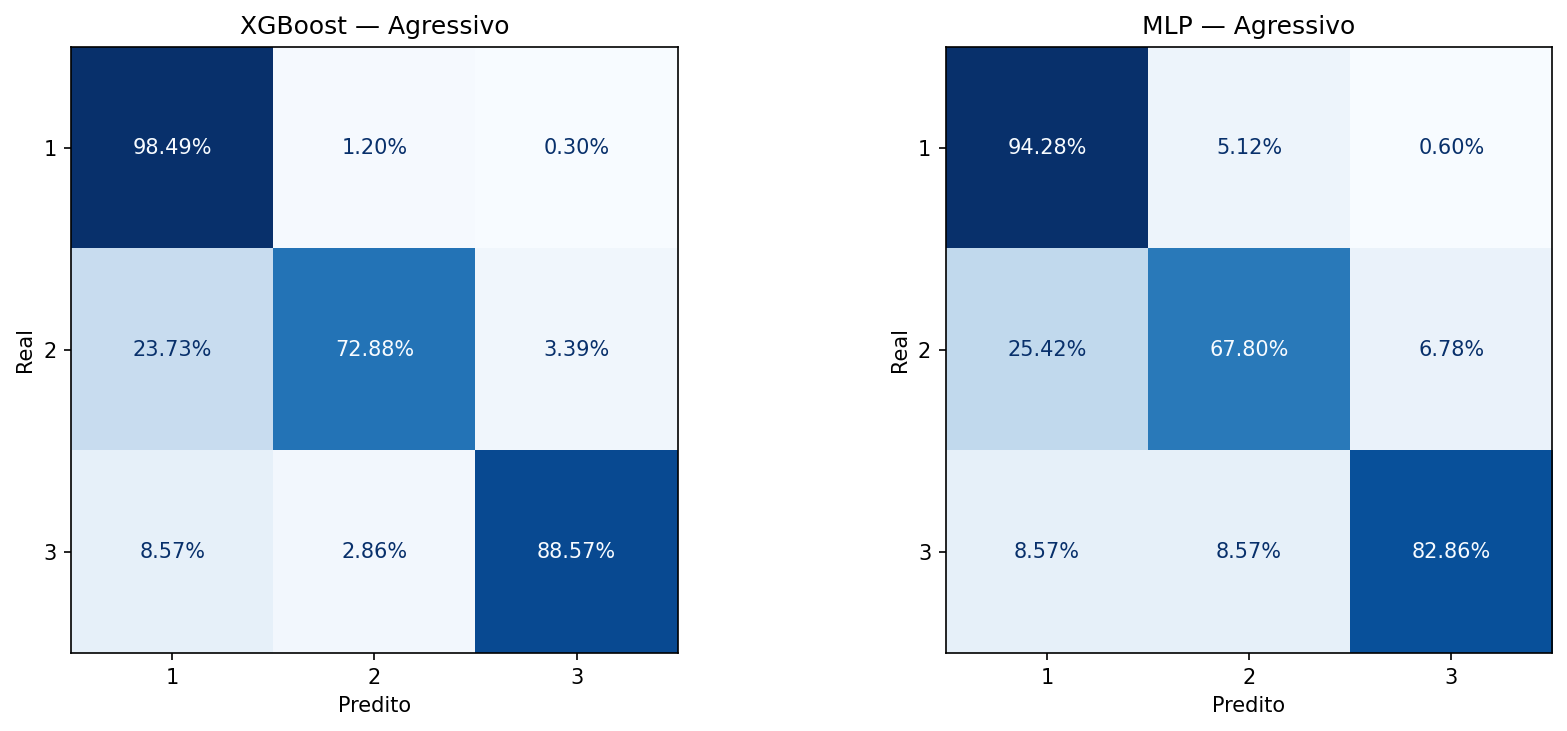
\includegraphics[width=0.85\textwidth]{Figures/matriz_confusao_agressivo.png}
\caption{Matrizes de confusão normalizadas (por linha) para XGBoost e MLP no dataset Agressivo.
Classes: 1 = Normal, 2 = Suspeito, 3 = Patológico.}
\label{fig:confusao}
\end{figure}

Ambos os modelos cometem erros predominantemente entre as classes \textit{Normal} e
\textit{Suspeito}. Isso é clinicamente aceitável, pois a fronteira entre essas duas categorias
é intrinsecamente ambígua. Os erros mais graves -- feto \textit{Normal} classificado como
\textit{Patológico} ou vice-versa -- são raros em ambos os modelos. O XGBoost manteve
revocação por classe acima de 73\% em todas as categorias, enquanto a MLP apresentou 68\% de
revocação na classe \textit{Suspeito}.

% ═══════════════════════════════  V – CONCLUSÃO  ════════════════════════════
\section{Conclusão}
\label{sec:conclusion}

Este trabalho apresentou um estudo comparativo entre dois modelos de Aprendizado de Máquina --
XGBoost e MLP -- para classificação automática da saúde fetal a partir de dados de
cardiotocografia. O processo incluiu análise exploratória, pré-processamento, seleção de
\textit{features} com três critérios distintos, busca de hiperparâmetros via \textit{Randomized Search}
com validação cruzada estratificada de 5 \textit{folds} e avaliação por seis métricas.

O XGBoost demonstrou desempenho superior em todos os cenários avaliados, alcançando F1-score
macro de até 0,8961 (dataset Conservador) e AUC-ROC de 0,9818, evidenciando alta capacidade
discriminativa mesmo em classes minoritárias. O dataset Agressivo (14 \textit{features}), com
desempenho praticamente equivalente ao melhor resultado, representa a configuração ideal para
implementação prática, pois alia robustez a menor custo computacional e maior potencial de
generalização.

A MLP, embora com desempenho inferior ao XGBoost, apresentou AUC-ROC acima de 0,95 em todos
os experimentos, indicando que o modelo aprende representações úteis do problema. O resultado
sugere que, com mais dados ou com técnicas de balanceamento como SMOTE, a MLP poderia se
aproximar do XGBoost em termos de F1-score nas classes minoritárias.

Como trabalhos futuros, destacam-se: (i) a aplicação de técnicas de balanceamento
(SMOTE, \textit{class weighting}) para melhorar o desempenho nas classes Suspeito e Patológico;
(ii) a investigação de modelos de aprendizado profundo (CNN, LSTM) sobre os sinais CTG brutos,
dispensando a extração manual de \textit{features}; (iii) a construção de um \textit{ensemble}
entre XGBoost e MLP para explorar a complementaridade das duas abordagens; e (iv) a validação
dos modelos em datasets externos para aferição da generalização real.

% ═══════════════════════════════  REFERÊNCIAS  ═══════════════════════════════
\bibliographystyle{plain}
\begin{thebibliography}{9}

\bibitem{who2020}
World Health Organization.
\textit{Newborns: improving survival and well-being}.
WHO Fact Sheet, 2020.
Disponível em: \url{https://www.who.int/news-room/fact-sheets/detail/newborns-reducing-mortality}.

\bibitem{campos2000}
Ayres-de-Campos, D.; Bernardes, J.; Costa-Pereira, A.; Pereira-Leite, L.
\textit{SisPorto 2.0: A Program for Automated Analysis of Cardiotocograms}.
Journal of Maternal-Fetal Medicine, v. 9, n. 5, p. 311--318, 2000.

\bibitem{hoodbhoy2019}
Hoodbhoy, Z.; Noman, M.; Shafique, A.; Nasim, A.; Chowdhury, D.; Hasan, B.
\textit{Use of Machine Learning Algorithms for Prediction of Fetal Risk using Cardiotocographic Data}.
International Journal of Applied and Basic Medical Research, v. 9, n. 4, p. 226--230, 2019.

\bibitem{subasi2020}
Subasi, A.; Kadasa, B.; Kremic, E.
\textit{Classification of the Cardiotocogram Data for Anticipation of Fetal Risks using Bagging Ensemble Classifier}.
Procedia Computer Science, v. 168, p. 34--39, 2020.

\bibitem{petrozziello2019}
Petrozziello, A.; Jordanov, I.; Chandraharan, E.; Redman, C. W.; Georgieva, A.
\textit{Deep learning for continuous electronic fetal monitoring in labor}.
In: \textit{41st Annual International Conference of the IEEE Engineering in Medicine and Biology Society (EMBC)}, p. 5872--5875, 2019.

\bibitem{rahman2022}
Rahman, A.; Hossain, M. S.; Alrajeh, N. A.; Gupta, B.
\textit{Fetal Health Classification from CTG Data using Ensemble Methods and Feature Importance Analysis}.
IEEE Access, v. 10, p. 33375--33389, 2022.

\bibitem{verma2021}
Verma, A. K.; Agrawal, S.; Shukla, B.
\textit{Feature Selection and Classification of Cardiotocography Data for Fetal Health Prediction}.
In: \textit{International Conference on Intelligent Communication, Control and Devices (ICICCD)},
Springer, p. 409--417, 2021.

\end{thebibliography}

\end{document}
